 
\section{Theory}
\subsection{Majorana Zero Modes and Topological Motivation}
Topological quantum computing is an approach to fault-tolerant quantum computation in which quantum gates are implemented by braiding non-Abelian anyons. The central idea is that information can be encoded non-locally in a degenerate subspace, so that local perturbations have limited access to the encoded quantum state. In this setting, the result of a gate depends on the topology of the braid rather than on microscopic details of the path.\\
Anyons are quasiparticles that, so far, have only been observed in effectively two-dimensional systems. In three spatial dimensions, identical particles are classified as either bosons or fermions, corresponding to symmetric and antisymmetric exchange statistics. In two dimensions, however, the topology of particle exchange allows for a richer possibility: exchanging two particles can produce statistics that are neither bosonic nor fermionic\\{\color{red}https://sciencex.com/wire-news/347971706/finally-anyons-reveal-their-exotic-quantum-properties.html}\\. In particular, exchanging two identical particles twice is not necessarily topologically equivalent to doing nothing, because the exchange path cannot always be continuously shrunk to a point without crossing another particle. Particles with such exchange statistics are called anyons, and they are classified as Abelian or non-Abelian depending on how the quantum state transforms under exchange. Abelian anyons acquire only a phase factor, while non-Abelian anyons transform the state within a degenerate subspace. This latter property is what makes non-Abelian anyons especially interesting for quantum computation{\color{red}https://www.nature.com/articles/nphys767}.\\ 
% \newpage
\begin{figure}[h]
  \begin{center}
      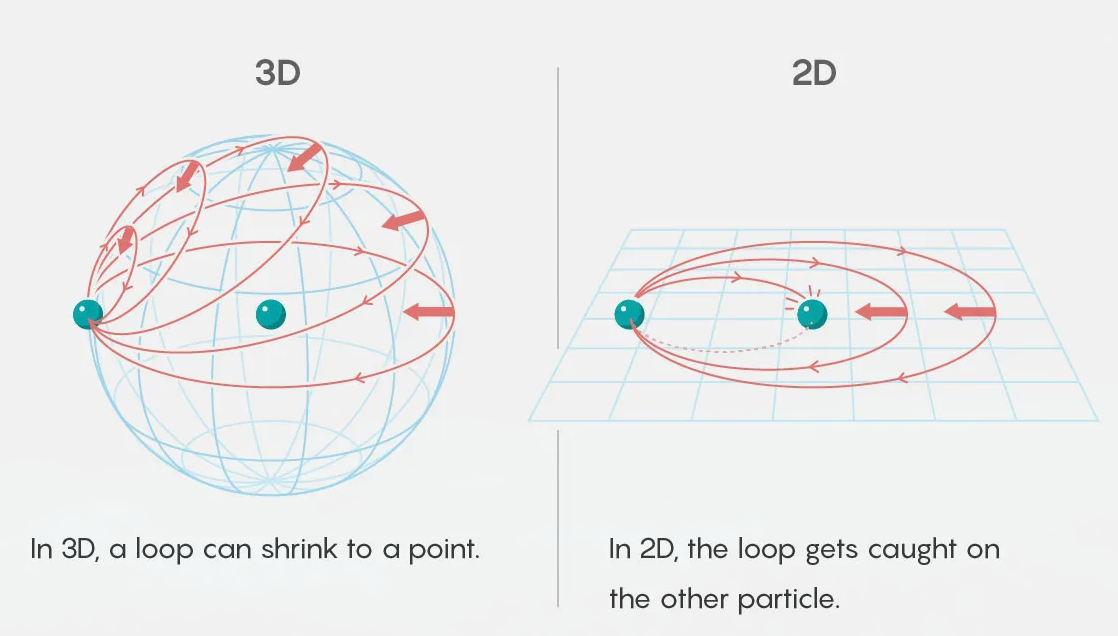
\includegraphics[width=0.8\textwidth]{figs/2d_v_3d_particle.png}
  \caption{Visualization of the difference between particle exchange in two and three dimensions. In three dimensions, the exchange loop can be shrunk to a point, making a double exchange topologically equivalent to leaving the particles unchanged. In two dimensions, the corresponding loop cannot be shrunk to a point without crossing the particle worldlines. This topological distinction allows anyons to exhibit non-trivial exchange statistics.{\color{red} $https://media.wired.com/photos/5ebf0488d58e99fafced8087/master/w_1600\%2Cc_limit/Science_Anyons-graphic-FINAL.jpg$}}
  \end{center}

  \label{fig:2d_v_3d_particle}
\end{figure}

A collection of non-Abelian anyons with fixed positions and fixed local quantum numbers can possess a non-trivial topological degeneracy. Quantum information can then be encoded in this degenerate subspace, while braiding the anyons implements unitary transformations within it. Since the resulting transformation depends only on the braid topology, and not on small local deformations of the path, this provides a possible route toward fault-tolerant quantum gates. In suitable schemes, braiding operations can be combined with additional ingredients to implement the gates needed for quantum computation.\\{\color{red}https://www.nature.com/articles/npjqi20151}\\ \\ 

One of the most promising candidates for realizing non-Abelian exchange statistics in condensed-matter systems is the Majorana zero mode (MZM), predicted to occur in certain topological superconductors. A Majorana zero mode is a zero-energy quasiparticle described by an operator that is equal to its own Hermitian conjugate. In one-dimensional topological superconductors, such modes can appear at the ends of the system. Unlike an ordinary fermionic mode, a single MZM can be viewed as ``half'' of a Dirac fermion: two Majorana operators can be combined to form one conventional fermionic operator,
\begin{equation}
    c = \frac{1}{2}(\gamma_1 + i\gamma_2)
\end{equation}
with the inverse relations
\begin{equation}
    \gamma_1 = c + c^\dagger, \qquad \gamma_2 = -i(c-c^\dagger).
\end{equation}
Here $\gamma_1$ and $\gamma_2$ are Majorana operators satisfying
\begin{equation}
    \gamma_i = \gamma_i^\dagger, \quad \{\gamma_i, \gamma_j\} = 2\delta_{ij}
\end{equation}
The non-Abelian character of MZMs is reflected in the fact that exchanging two of them produces a non-trivial unitary transformation on the degenerate ground-state manifold{\color{red}https://www.nature.com/articles/npjqi20151}.\\ 
The primary motivation for studying MZMs and their braiding properties is their combination of non-local encoding and spectral protection. When a fermionic state is formed from two spatially separated MZMs, local environmental noise cannot easily determine or flip the encoded state, because such an error would require coupling to both separated Majorana components. Therefore, local perturbations are strongly suppressed as a source of decoherence{\color{red}https://journals.aps.org/rmp/abstract/10.1103/RevModPhys.80.1083}.\\
MZMs also give rise to ground-state degeneracies. A system with $2n$ Majorana zero modes spans a $2^n$-dimensional fermionic Hilbert space associated with the occupations of $n$ non-local fermions. If the total fermion parity is fixed, the physical ground-state degeneracy is reduced to $2^{n-1}$. In either case, the useful low-energy manifold must be separated from excited states by a finite spectral gap, which protects the encoded information against thermal excitations.{\color{red}https://arxiv.org/abs/cond-mat/0010440}.\\
The remaining question is how such Majorana operators can emerge from an ordinary fermionic Hamiltonian. The Kitaev chain provides the minimal model where this mechanism can be seen explicitly, and it also gives the conceptual starting point for the Poor Man's Majorana systems studied in this thesis.





\subsection{Kitaev Chain and Poor Man's Majorana Systems}
Before discussing the Majorana models used in this thesis, we first introduce their theoretical origin: the Kitaev chain. The Kitaev chain, or Kitaev-Majorana chain, is a simplified model for a topological superconductor. First proposed by Alexei Kitaev in 2000 {\color{red}https://arxiv.org/pdf/cond-mat/0010440}, the Kitaev chain is a one-dimensional superconducting system that can host Majorana zero modes at its ends under certain conditions, illustrated in Figure~\ref{fig:kitaev}. The model is defined on a lattice of spinless fermions with nearest-neighbor hopping and superconducting pairing. 
The Hamiltonian of the Kitaev chain is
\begin{equation}
H = -\mu \sum_{j=1}^{N} \left(c_j^\dagger c_j - \frac{1}{2}\right)
- t \sum_{j=1}^{N-1} \left(c_j^\dagger c_{j+1} + c_{j+1}^\dagger c_j\right)
+ \Delta \sum_{j=1}^{N-1} \left(c_j c_{j+1} + c_{j+1}^\dagger c_j^\dagger\right),
\label{eq:kitaev_ham}
\end{equation}
Each term in Eq.~\ref{eq:kitaev_ham} has a clear physical interpretation. The first term represents the chemical potential $\mu$, which controls the filling of the fermionic states. The second term describes the hopping of fermions between neighboring sites with amplitude $t$. The third term represents $p$-wave superconducting pairing, where pairs of fermions are created or annihilated on adjacent sites with amplitude $\Delta$.\\
As shown schematically in Fig.~\ref{fig:kitaev}, the Kitaev chain has two distinct phases depending on the parameters $\mu$, $t$, and $\Delta$. In the trivial phase, the Majorana modes on the same site pair up to form conventional fermions, leaving no unpaired modes. In the topological phase, Majoranas on adjacent sites couple, leaving unpaired modes at the chain ends. These unpaired Majoranas combine into a non-local fermionic mode that can be occupied or empty without costing energy, leading to a twofold degeneracy in the ground state. This degeneracy is protected as long as local perturbations do not close the bulk gap or directly hybridize the edge modes.\\



\begin{figure}
  \centering
  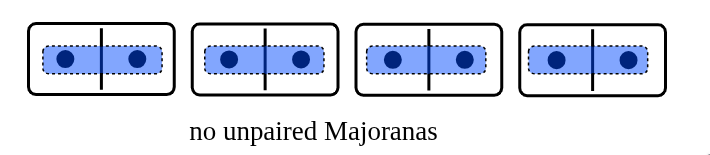
\includegraphics[width=0.45\textwidth]{figs/no_unpaired.png}
  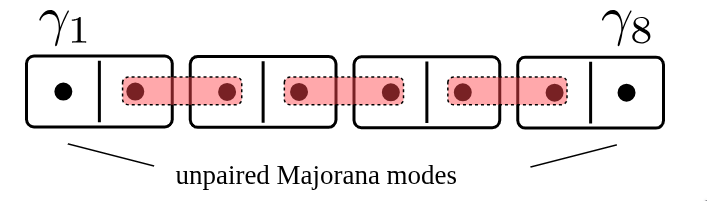
\includegraphics[width=0.45\textwidth]{figs/unpaired.png}
  \caption{Schematic representation of the Kitaev chain in its two distinct phases. Left: In the trivial phase, Majorana modes on the same site pair to form conventional fermions, leaving no unpaired modes. Right: In the topological phase, Majoranas on adjacent sites couple, leaving unpaired modes at the chain ends, which combine into a non-local fermionic mode. {\color{red}Topocondmat}}
  \label{fig:kitaev}
\end{figure}

The topological phase of the Kitaev chain is the basic model for the Majorana zero modes studied in this thesis. The goal is then to understand how similar Majorana-like physics can be engineered in more realistic systems.
\\ \\

\paragraph{Bulk Spectrum and Topological Phase\newline}

In order to determine when the Kitaev chain is topological, we need to consider the properties of the bulk spectrum. \\ 
For a translationally invariant chain, we can perform a Fourier transform to momentum space, which allows us to analyze the energy spectrum and identify the conditions for the topological phase. The Fourier transform is given by

\begin{equation}
  c_j = \frac{1}{\sqrt{N}} \sum_p e^{ipaj} c_p
\end{equation}
This transformation allows the Hamiltonian to be expressed in terms of momentum-space operators $c_p$ and $c_p^\dagger$. The resulting Hamiltonian in momentum space is
\begin{equation}
H = ∑_{ p}^{} ξ_p\left(c_p^{†} c_p - \frac{1}{2}\right) - ∑_{p}^{} t \cos p a + Δ ∑_{p}^{}\left(c_p^{†} c_{-p}^{†} e^{ipa} + c_{-p} c_p e^{-ipa}\right), 
\end{equation}

with $ξ_p = -μ - 2t \cos pa$ and $a$ being the lattice spacing. In the Bogoliubov--de Gennes formalism, the quasiparticle spectrum becomes
\begin{equation}
  E_{p,\pm} = \pm \sqrt{(\mu + 2t \cos{pa})^2 + 4\Delta^2 \sin^2{pa}}.
\end{equation}
Even though the Bogoliubov--de Gennes formalism describes a non-interacting quasiparticle problem, it still provides the basic topological picture that the interacting models in this thesis build on. In Fig.~\ref{fig:kitaev_bands}, we can see how the spectrum changes as the chemical potential $\mu$ is tuned. The presence of a gap is crucial for the stability of the Majorana modes, and the closing and reopening of this gap signals a topological phase transition.\\ \\
The quasiparticle spectrum is gapped for most parameter values, but the gap closes when
\[
|\mu| = 2|t|.
\]
This is also visible in Fig.~\ref{fig:kitaev_bands}. The gap closing marks the transition between the trivial and topological phases. When $\mu$ crosses this boundary, the ground state changes its topological character without requiring ordinary symmetry breaking {\color{red}Qtech}.\\
\begin{figure}
  \centering
    
    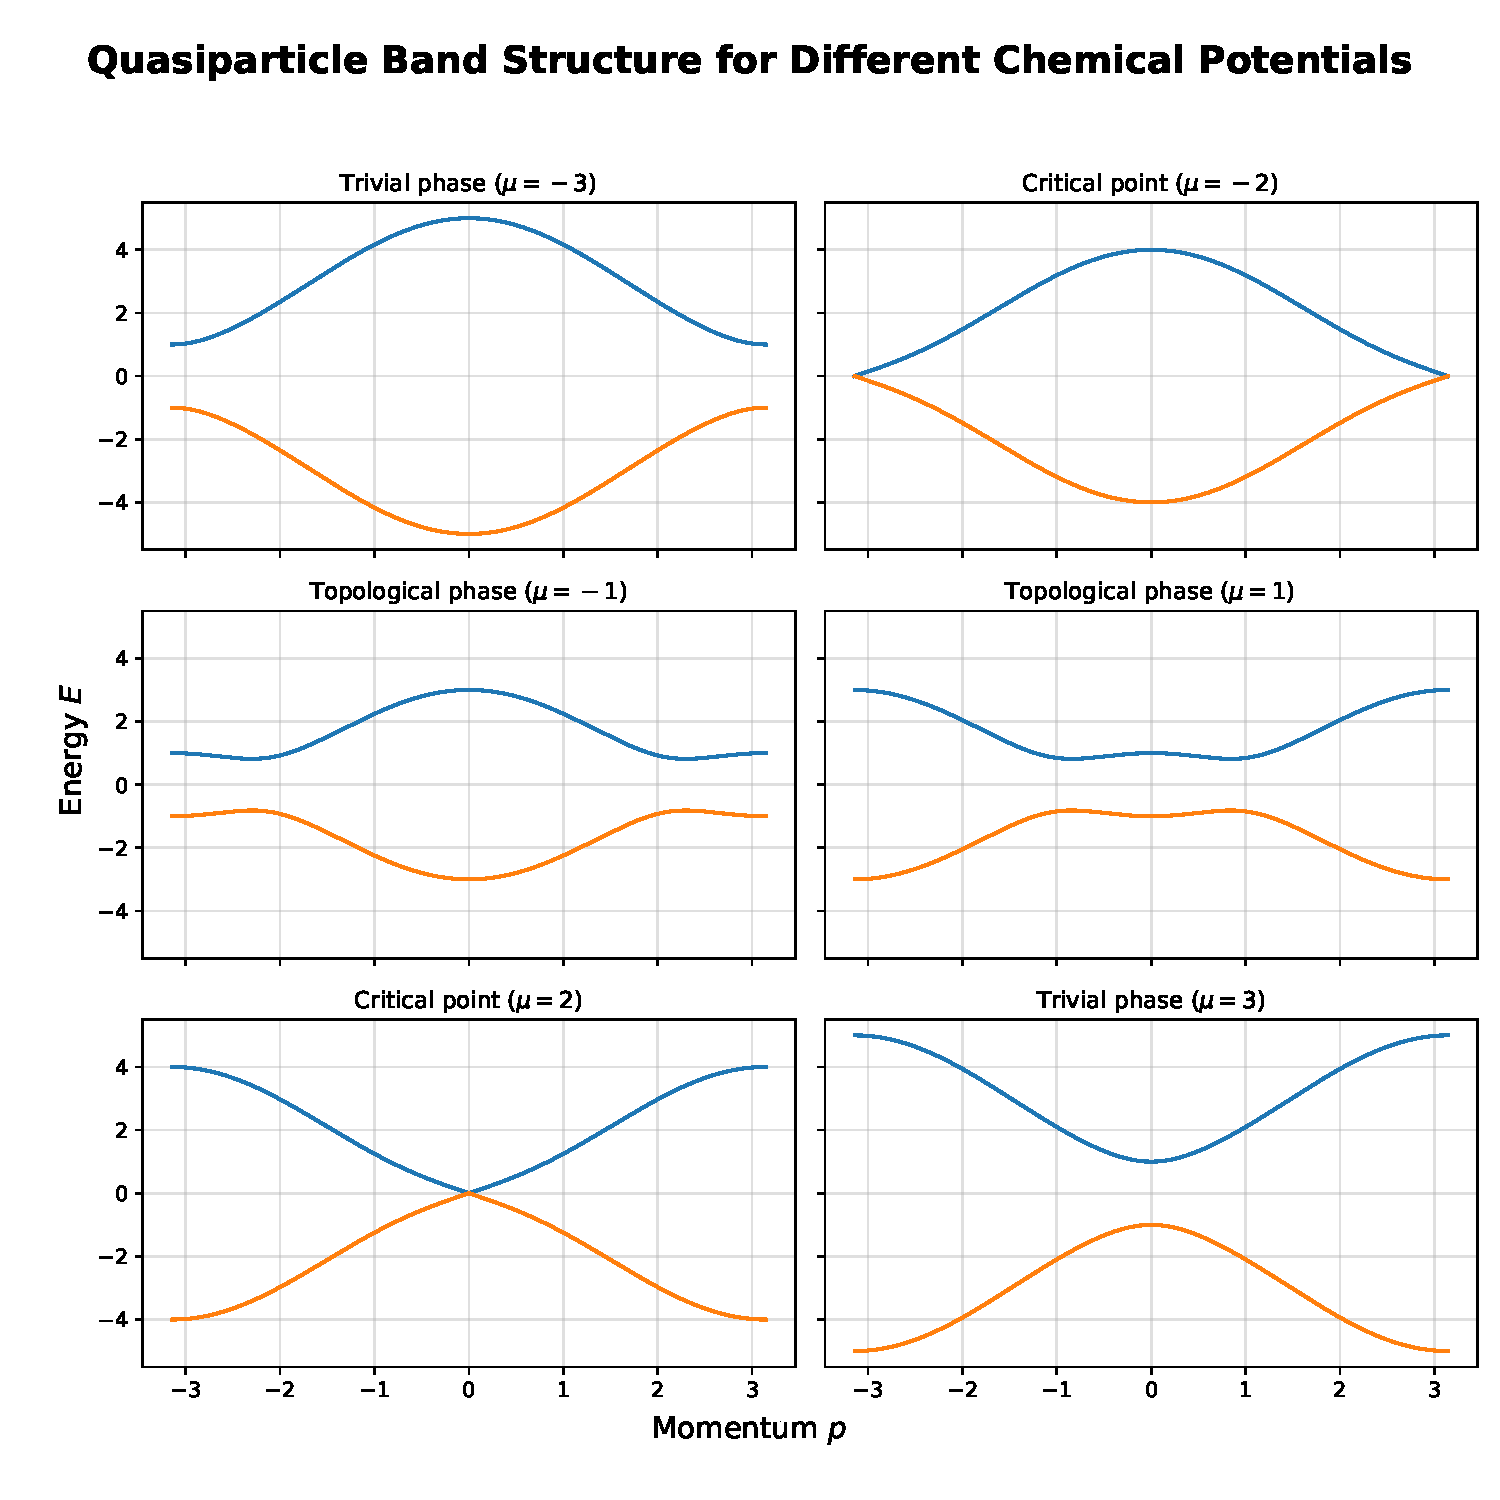
\includegraphics[width=.8\textwidth]{figs/band_structure.pdf}
    \caption{Quasiparticle energy spectrum of the Kitaev chain for different chemical potentials $\mu$. Left: In the trivial phase ($|\mu| > 2|t|$), the spectrum is fully gapped with no zero-energy modes. Right: In the topological phase ($|\mu| < 2|t|$), the gap closes and reopens, signaling the emergence of zero-energy edge modes.}
  \label{fig:kitaev_bands}
\end{figure}
\newpage

\paragraph{Majorana Representation and Zero Modes\newline}
Looking back at Fig.~\ref{fig:kitaev}, we want a representation that makes the unpaired edge modes more explicit. To do so, we express the fermionic operators in terms of Majorana operators. For each site $j$, we define two Majorana operators $\gamma_j^A$ and $\gamma_j^B$ as follows:
\begin{equation}
c_j = \frac{1}{2}(\gamma_j^A + i\gamma_j^B), \quad
c_j^\dagger = \frac{1}{2}(\gamma_j^A - i\gamma_j^B),
\label{eq:first_majorana_rep}
\end{equation}
where $\gamma_j^{A,B}$ satisfy $\{\gamma_j^\alpha, \gamma_k^\beta\} = 2\delta_{jk}\delta_{\alpha\beta}$ and $(\gamma_j^\alpha)^\dagger = \gamma_j^\alpha$. In the trivial phase, the Majorana operators pair on the same site. In the topological phase, and especially at the ideal point $t=\Delta$ and $\mu=0$, $\gamma_j^B$ couples to $\gamma_{j+1}^A$. This leaves two edge modes unpaired, $\gamma_1^A$ and $\gamma_N^B$, at the chain ends. These two unpaired Majoranas define a non-local fermionic mode,
\begin{equation}
  f = \frac{1}{2}(\gamma_1^A + i\gamma_N^B),
\end{equation}
which satisfies $\{f, f^\dagger\}=1$ and costs zero energy to occupy. This non-local fermionic mode creates the basis for the exploration of Majorana physics in this thesis, and it is the key to understanding how Majorana modes can be used for quantum computation. The occupation of this non-local mode corresponds to a twofold degeneracy in the ground state, which is protected as long as local perturbations do not close the bulk gap or directly hybridize the two edge modes. This non-local encoding of information is what gives Majorana modes their potential for fault-tolerant quantum computation, as local errors cannot easily access or change the encoded state.{\color{red}Qtech}


\paragraph{Poor Man's Majorana Systems\newline}

While the Kitaev chain is the minimal theoretical model, it assumes spinless fermions and intrinsic $p$-wave pairing. Real superconductors are usually spinful and dominated by conventional $s$-wave pairing. The Poor Man's Majorana (PMM) platform is a compact engineered system whose low-energy behavior can mimic a short Kitaev chain. The simplest version is a double quantum dot coupled through a superconducting segment. Each dot acts as a site, elastic cotunneling produces effective hopping, and crossed Andreev reflection produces an effective non-local pairing term.\\

The effective two-dot Hamiltonian can be written as
\begin{equation}
H = \sum_{i=L,R} \epsilon_i n_i
+ t (d_L^\dagger d_R + d_R^\dagger d_L)
+ \Delta (d_L^\dagger d_R^\dagger + d_R d_L)
+ U n_L n_R,
\label{eq:qdsqdh}
\end{equation}
where $d_{L/R}^\dagger$ and $d_{L/R}$ are creation and annihilation operators on the left and right dots, $n_i$ is the number operator, $\epsilon_{L,R}$ are the dot energy levels, $t$ is the elastic cotunneling amplitude, $\Delta$ is the crossed Andreev reflection amplitude, and $U$ is the interdot Coulomb interaction energy. The parameters map directly onto the Kitaev-chain language:
\begin{itemize}
    \item \textbf{Elastic cotunneling (ECT):} An electron tunnels coherently from one dot to the other through a virtual process in the superconductor. This produces the effective hopping amplitude $t$.
    \item \textbf{Crossed Andreev reflection (CAR):} A Cooper pair splits, with one electron entering each dot. This produces the non-local pairing amplitude $\Delta$.
    \item \textbf{On-site energy:} The dot energies $\epsilon_L$ and $\epsilon_R$ play the role of local chemical potentials.
\end{itemize}
At the ideal non-interacting sweet spot, $|\epsilon_L|=|\epsilon_R|=0$ and $|t|=|\Delta|$, the two-dot system develops Majorana-like states localized primarily on opposite dots. Since the system is finite and lacks a true bulk, these states are not topologically protected in the same sense as an infinite Kitaev chain. This is why they are referred to as Poor Man's Majoranas {\color{red}Qtech}.\\

For the purposes of this thesis, the PMM idea is generalized from two dots to interacting $n$-dot chains. A schematic representation is shown in Figure \ref{fig:PMM_setup}. Adding more dots introduces more tunable parameters and more possible low-energy structure, but it also makes the analytic sweet-spot problem much harder. This motivates the numerical optimization strategy discussed later in the thesis.
\begin{figure}
  \centering
  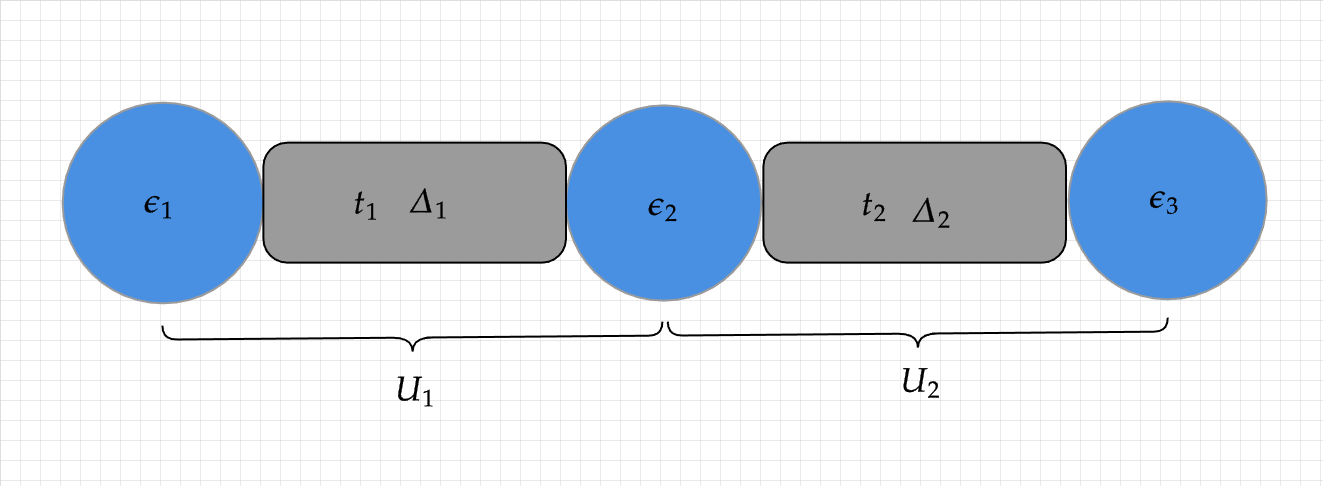
\includegraphics[width=0.8\textwidth]{figs/PMMSetup.png}
  \caption{Schematic representation of the PMM setup. The three quantum dots are represented by the blue circles, and the superconducting segments are represented by the grey rectangles. The tunable parameters of the system, such as the dot energy levels, ECT, CAR and the Coulomb interaction, are indicated by their respective labels. By tuning these parameters, we can access different regimes of the system and identify the sweet spots where Majorana-like modes emerge.}
  \label{fig:PMM_setup}
\end{figure}

\subsection{Diagnostics of Majorana-like States}
In a finite PMM system, the presence of low-energy states alone is not enough to claim Majorana physics. The states must also have the right parity structure, local indistinguishability, charge distribution, and Majorana-polarization profile. These diagnostics are especially important in interacting systems, where a low numerical energy splitting can appear for reasons that are not necessarily related to edge-localized Majorana modes.\\

\paragraph{Fermion Parity\newline}
The mean-field Hamiltonian of a superconductor does not conserve particle number, because particles can be added or removed in Cooper pairs. It does, however, conserve fermion parity. The parity operator can be written as
$$
P = (-1)^{N} = Π_n(1 - 2c_n ^{†} c_n),
$$
where $N$ is the total particle number. The eigenvalues of $P$ are $+1$ for even parity and $-1$ for odd parity. In a Majorana system, the two lowest states often differ by fermion parity, and near-degeneracy between these opposite-parity states is one of the central signatures of a Majorana-like mode {\color{red}Topocondmat}.\\

\paragraph{Energy Degeneracy and Spectral Gap \newline}
The first spectral signature is approximate degeneracy between even- and odd-parity states. In the ideal case, the ground states in the two parity sectors are exactly degenerate. In practice, a finite system will generally have a small splitting, and the goal is to make this splitting as small as possible compared with the excitation gap. The gap to higher excited states is also crucial: it protects the low-energy manifold from thermal excitations and helps justify projecting the dynamics onto a small subspace during braiding.{\color{red}Topocondmat}\\
\begin{figure}
  \centering
  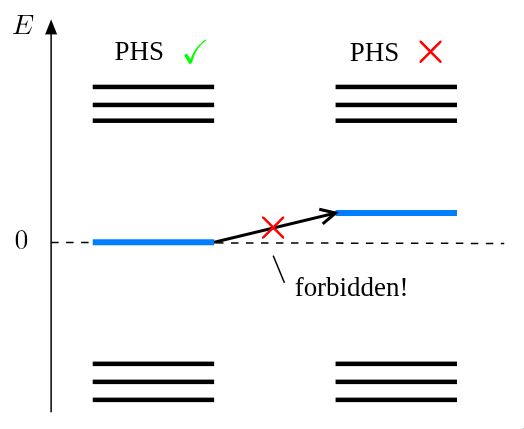
\includegraphics[width=0.5\textwidth]{figs/gs_symmetry}%
  \caption{Energy spectrum showing how the energy eigenvalues of the system must be symmetric around zero energy due to particle-hole symmetry \cite{Topocondmat}.}
  \label{fig:gs_symmetry}
\end{figure}

\paragraph{Local Distinguishability\newline}
A defining feature of spatially separated Majorana modes is that the encoded information is non-local. Local measurements should therefore not reveal whether the system is in the even or odd ground state. One way to quantify this is through the local distinguishability parameter
$$
\text{LD} = \frac{1}{N} \sum_{j=1}^{N} || \rho_j^o - \rho_j^e || = \frac{1}{N} \sum_{j=1}^{N} || \delta \rho_j ||.
$$
{\color{red}Lund1, VikMar}.
Here, $\rho_j^{o/e}$ are the reduced density matrices of site $j$ for the odd and even parity ground states, respectively, and $||\cdot||$ is the trace norm. A value close to zero indicates that the two states are locally indistinguishable, while a larger value indicates that local measurements can tell the two parity states apart.\\

\paragraph{Majorana Polarization\newline}
The Majorana polarization (MP) is used to quantify how closely the low-energy states resemble spatially localized Majorana modes. In an ideal PMM configuration, the polarization should be concentrated at the edge dots, with opposite signs on the two ends and little or no weight in the bulk. One useful definition is
$$
M_\alpha = \frac{W_\alpha^2 - Z_\alpha^2}{W_\alpha^2 + Z_\alpha^2},
$$
where
$$
W_\alpha = ∑_{\sigma} \bra{o} c_{\alpha\sigma} + c_{\alpha\sigma}^{†} \ket{e}, \quad Z_\alpha = i ∑_{\sigma} \bra{o} c_{\alpha\sigma} - c_{\alpha\sigma}^{†} \ket{e}.
$$
Here, $\alpha$ denotes the site index, $\sigma$ is the spin index, and $\ket{o}$ and $\ket{e}$ are the odd- and even-parity ground states. In an ideal sweet spot with two perfectly localized Majoranas, the edge values would satisfy $M_L=-M_R=\pm 1$ \cite{Qtech}.\\

\paragraph{Charge Expectation and Non-locality\newline}
Another diagnostic is the local charge expectation value in the even and odd states,
$$
\bra{e}n_{L(R)} \ket{e}, \quad \bra{o}n_{L(R)} \ket{o}.
$$
In the ideal case, these expectation values should be equal for the two parity states. A small charge difference means that the two states share the same local charge distribution, which is another way of saying that the parity information is stored non-locally rather than being visible on a single dot.\\

\paragraph{Optimization Motivation\newline}
For a simple two-dot system, the relevant tunable parameters are the dot energies, elastic cotunneling, crossed Andreev reflection, and interaction strength. For longer chains, the number of tunable parameters grows quickly. Since interactions and inhomogeneous parameters make it difficult to identify sweet spots analytically, the diagnostics above can be combined into a loss function and used to search numerically for promising Majorana-like regimes. The resulting loss landscape may contain many local minima, which motivates the repeated-restart and basin-hopping strategy described in the methods chapter.
\begin{figure}
\centering
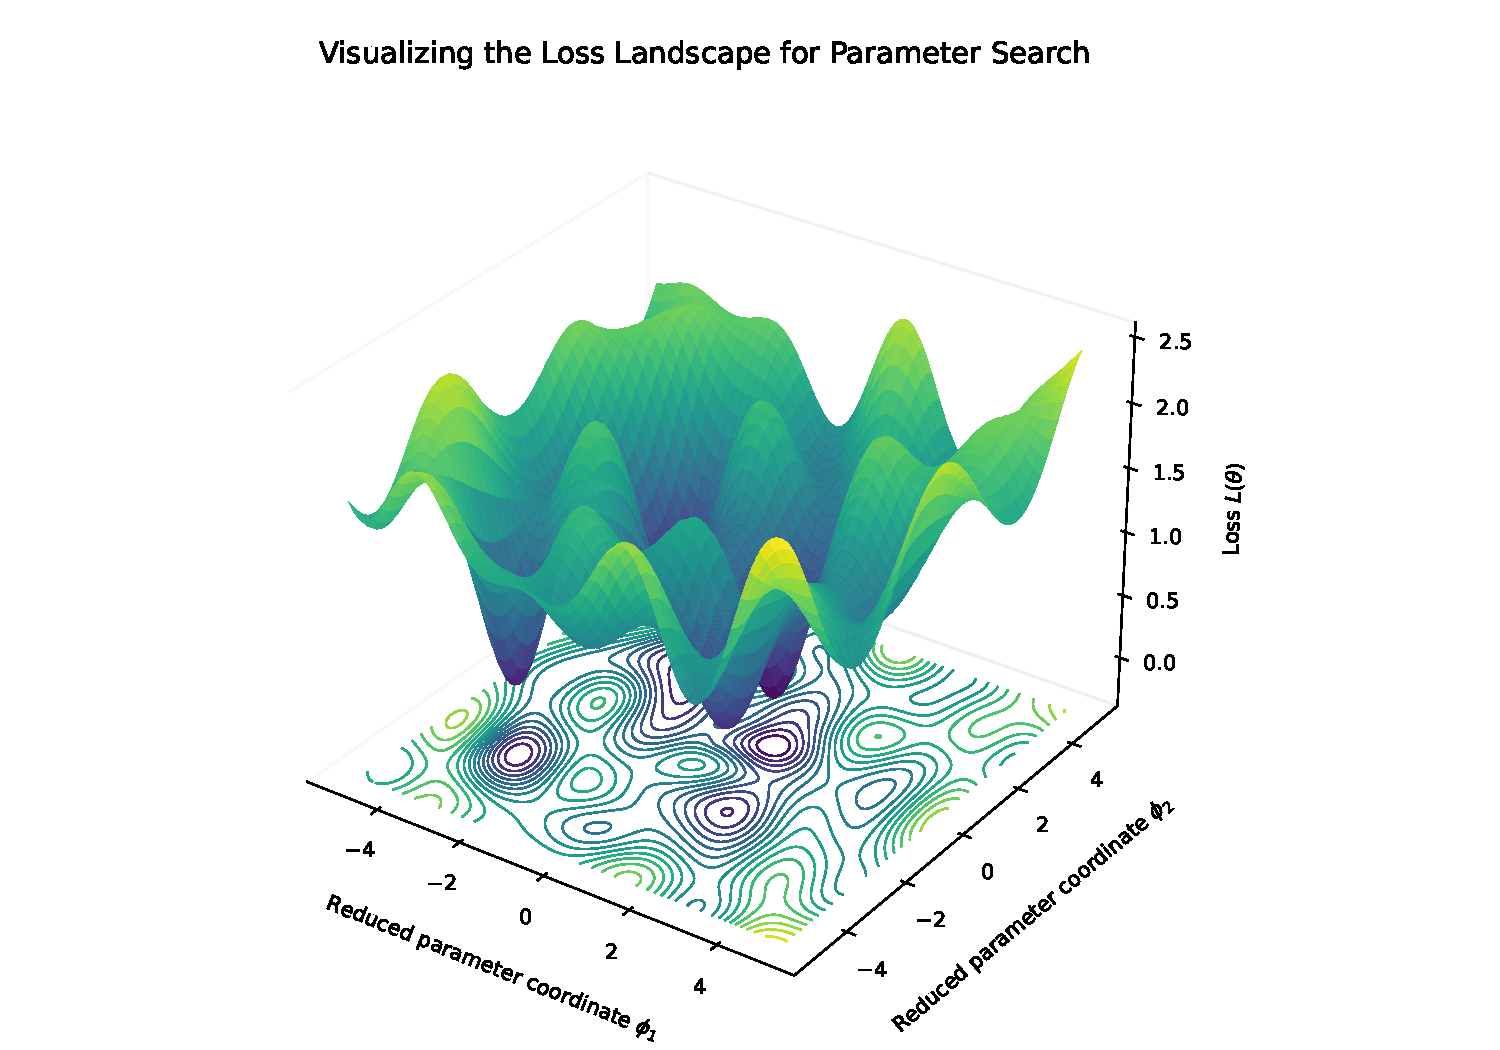
\includegraphics[width=\textwidth]{figs/3dparametersearch.pdf}
\caption{Visualization of the parameter space for an n-dot system, showing how multiple parameters and their combinations create a complex landscape with multiple local minima.}
\label{fig:paramVisualization}
\end{figure}

\subsection{Majorana Exchange and Braiding}
Braiding is the operation that makes Majorana modes useful for topological quantum computation. The basic idea is to exchange two Majorana modes adiabatically so that the quantum state transforms according to their non-Abelian statistics. Because the transformation is tied to the topology of the exchange, rather than to the exact microscopic path, braiding offers a route to gates that are less sensitive to local control errors. Braiding in the right patterns, with the right systems, can lead to the implementation of useful quantum gates.{\color{red} SOURCE}\\

\subsubsection{Quantum Gates}
In the circuit model of quantum computation, a gate is a unitary operation acting on one or more qubits. The Pauli gates are among the simplest examples:
\begin{equation}
X = \begin{pmatrix} 
0 & 1 \\
1 & 0
\end{pmatrix}, \quad
Y = \begin{pmatrix}
0 & -i \\
i & 0
\end{pmatrix}, \quad
Z = \begin{pmatrix}
1 & 0 \\
0 & -1
\end{pmatrix}.
\end{equation}
Acting on the basis states
\begin{equation}
\ket{0} = \begin{pmatrix}
1 \\
0
\end{pmatrix}, \quad
\ket{1} = \begin{pmatrix}
0 \\
1
\end{pmatrix},
\end{equation}
these gates produce
\begin{align*}
X\ket{0} &= \ket{1}, \quad X\ket{1} = \ket{0}, \\
Y\ket{0} &= i\ket{1}, \quad Y\ket{1} = -i\ket{0}, \\
Z\ket{0} &= \ket{0}, \quad Z\ket{1} = -\ket{1}.
\end{align*}
\begin{figure}
  \centering
  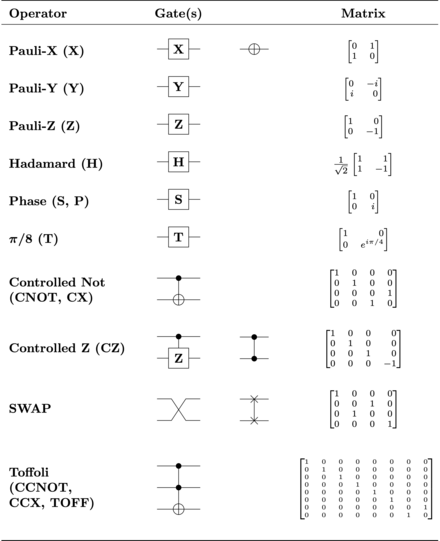
\includegraphics[width = 0.5\textwidth]{figs/Quantum_logic_gates.png}
  \label{fig:quantum_gates}
    \caption{List of common quantum gates and their matrix representations. {\color{red} Wikipedia Quantum logic gates}}
\end{figure}

\paragraph{Pauli Gates in Fermionic Language}
To connect gates to Majorana systems, it is useful to express simple qubit operations in terms of fermionic operators. For a two-site system with fermionic operators $c_1$ and $c_2$, one can write
\begin{align*}
  X &= c_1 ^{†} c_2 + c_2 ^{†} c_1, \\
  Y &= -i(c_1 ^{†} c_2 - c_2 ^{†} c_1), \\
  Z &= c_1 ^{†} c_1 - c_2 ^{†} c_2.
\end{align*}
These expressions show how qubit operations can be represented through hopping-like and occupation-like operators in a fermionic system.\\

\subsubsection{Jordan-Wigner Transformation}
The Jordan-Wigner transformation maps spin operators to fermionic creation and annihilation operators. Starting from
\begin{align*}
\sigma_j^+ &= \frac{1}{2}(\sigma_j^x + i\sigma_j^y) \equiv f_j ^{†}, \\
\sigma_j^- &= \frac{1}{2}(\sigma_j^x - i\sigma_j^y) \equiv f_j, \\
\sigma_j^z &= 2f_j ^{†} f_j - 1,
\end{align*}
the same-site fermionic relation is correct, but operators on different sites commute instead of anticommute. To fix this, one introduces a string of $\sigma^z$ operators,
\begin{equation}
  a_j^{†} = Π_{k=1}^{j-1} (-\sigma_k^z) \cdot f_j^{†}, \quad a_j = Π_{k=1}^{j-1} (-\sigma_k^z) \cdot f_j,
\end{equation}
which gives
\begin{align*}
\{a_j^{†}, a_k\} &= \delta_{jk}, \\
\{a_j^{†}, a_k^{†}\} &= 0, \\
\{a_j, a_k\} &= 0.
\end{align*}
{\color{red} SOURCE JW WIKIPEDIA}\\

\paragraph{Pauli Matrices in the Majorana Representation}
Using the Majorana representation from Eq.~\ref{eq:first_majorana_rep}, define four Majorana operators by
\begin{align*}
  c_1 &= (\gamma_0 + i \gamma_1)/2, \quad c_1 ^{†} = (\gamma_0 - i \gamma_1)/2, \\
  c_2 &= (\gamma_2 + i \gamma_3)/2, \quad c_2 ^{†} = (\gamma_2 - i \gamma_3)/2.
\end{align*}
The Pauli operators can then be expressed as Majorana bilinears. In a fixed parity subspace, these simplify to
\begin{align*}
  X &= \frac{i}{2} (\gamma_0\gamma_3 - \gamma_1\gamma_2) = i\gamma_0\gamma_3 = -i\gamma_1\gamma_2, \\
  Y &= -\frac{i}{2} (\gamma_0\gamma_2 + \gamma_1\gamma_3) = -i \gamma_0\gamma_2 = -i \gamma_1\gamma_3, \\
  Z &= \frac{i}{2} (\gamma_0\gamma_1 + \gamma_2\gamma_3) = i\gamma_0\gamma_1 = i\gamma_2\gamma_3.
\end{align*}
This is the key connection between qubit gates and Majorana couplings: turning on controlled bilinear couplings between Majoranas implements rotations in the encoded qubit space.\\

\paragraph{Majorana Exchange Gates}
The unitary operator associated with exchanging two Majoranas $\gamma_i$ and $\gamma_j$ should satisfy
\begin{align*}
B_{ij} \gamma_i B_{ij} ^{†} &= \gamma_j, \\
B_{ij} \gamma_j B_{ij} ^{†} &= -\gamma_i, \\
B_{ij} \gamma_k B_{ij} ^{†} &= \gamma_k \quad \text{for } k \neq i,j.
\end{align*}
The corresponding exchange operator can be written as
\begin{equation}
B_{ij} = \frac{i}{\sqrt{2}} (1 - \gamma_i \gamma_j), \quad B_{ij} ^{†} = \frac{1-i}{\sqrt{2}} (1 + \gamma_i \gamma_j).
\end{equation}
Squaring exchange operations gives transformations directly related to Pauli gates:
\begin{align*}
B_{12}^2 &= -i\gamma_1\gamma_2 = -X, \\
B_{03}^2 &= i\gamma_0\gamma_3 = X, \\
B_{02}^2 &= i\gamma_0\gamma_2 = -Y,\\
B_{13}^2 &= i\gamma_1\gamma_3 = -Y,\\
B_{01}^2 &= i\gamma_0\gamma_1 =  Z,\\
B_{23}^2 &= i\gamma_2\gamma_3 =  -Z.
\end{align*}

\subsection{Projected Subspaces, Kato Transport and Braid Unitaries}
\subsubsection{Kato Berry Phase}
The Berry phase is a geometric phase acquired by a quantum state during adiabatic evolution around a closed loop in parameter space. For a non-degenerate eigenstate, the state returns to itself up to a phase. This phase has a dynamical part, which depends on the time scale and the energy of the state, and a geometric part, which depends only on the path in parameter space. The geometric contribution is the Berry phase.\\

For a degenerate subspace, the situation is richer. The adiabatic evolution can mix states within the degenerate manifold, so the Berry phase becomes a matrix rather than a scalar phase. In this thesis, this non-Abelian Berry matrix is what determines the braid unitary acting on the Majorana qubit space.\\

The Kato formulation provides a convenient way to compute this adiabatic transport. Instead of tracking individual eigenvectors and their phases, one works directly with the projector $P(t)$ onto the relevant low-energy subspace. The Kato evolution satisfies
$$
\partial_{t}U_t = i \left[P, \partial_{t}P\right]U_t, \qquad
U_0 = I.
$$
The final unitary $U_T$ is the non-Abelian Berry phase associated with the path. In numerical calculations, $P(t)$ is obtained by diagonalizing the Hamiltonian at each time step and constructing the projector onto the chosen low-energy manifold.\\

\subsubsection{Effective Braiding Hamiltonian}
As a reference model, assume that the system contains four Majorana modes $\gamma_0$, $\gamma_1$, $\gamma_2$, and $\gamma_3$ involved in the braid. A useful physical picture is a Y-junction made from three PMM subsystems, where one central Majorana is coupled sequentially to different neighboring Majoranas.\\
\begin{figure}
  \centering
  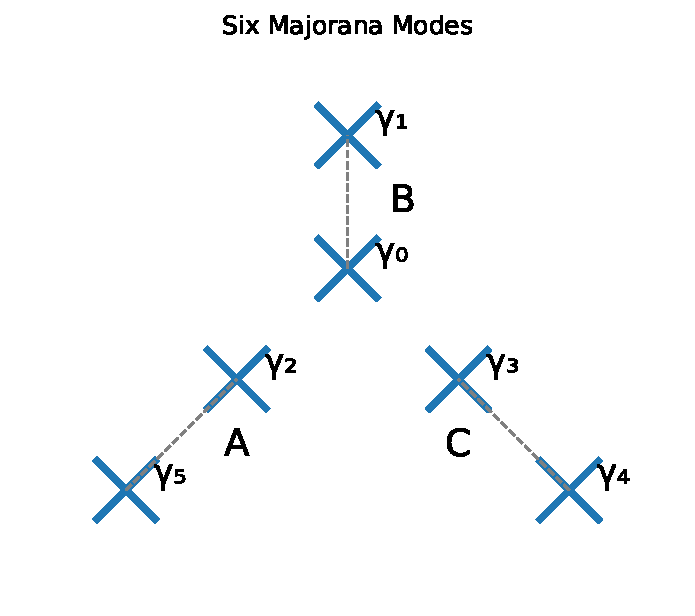
\includegraphics[width=0.5\textwidth]{figs/sixmajoranas.pdf}
  \caption{Schematic representation of a system hosting six majoranas. The illustrations shows pairs of two and two Majoranas coupling together, in a Y-junction, each pair form a subsystem that can be described by a Poor Man’s Majorana setup, A, B and C.}
  \label{fig:6_majoranas}
\end{figure}
In Fig.~\ref{fig:6_majoranas}, the four Majoranas $\gamma_0$, $\gamma_1$, $\gamma_2$, and $\gamma_3$ are the modes actively used in the braid, while $\gamma_4$ and $\gamma_5$ form a spectator pair. The ideal effective Hamiltonian can be written as
\begin{equation}
  \begin{aligned}
    H = &\Delta_{01} i\gamma_0\gamma_1 + \\
    &\Delta_{02} i\gamma_0\gamma_2 + \\
    &\Delta_{03} i\gamma_0\gamma_3,
  \end{aligned}
  \label{eq:H_eff}
\end{equation}
where $\Delta_{ij}$ is a tunable coupling between Majoranas $\gamma_i$ and $\gamma_j$. By turning these couplings on and off in a controlled sequence, the system can implement an effective exchange operation.\\

In a microscopic PMM device, the tunable quantities are not abstract Majorana bilinears, but physical hopping and pairing couplings between dots or subsystems. A junction between two PMM subsystems can be modeled by
\begin{equation}
  H_{JuncAB} = t_{AB} (d_{A} ^{†} d_{B} + d_{B} ^{†} d_{A}) + \Delta_{AB} (d_{A} ^{†} d_{B} ^{†} + d_{B} d_{A}),
  \label{eq:junctionHamiltonian}
\end{equation}
which is the same type of elastic cotunneling and crossed-Andreev pairing structure appearing in the PMM Hamiltonian. This motivates comparing two related braid constructions: one built from ideal or energy-level Majorana operators, and one built from projected microscopic local operators.\\

\subsubsection{Energy-Level and Local-Operator Braids}
The energy-level construction starts from the parity-resolved eigenstates of each optimized subsystem. Even and odd states are paired by energy, and effective Majorana operators are formed from combinations such as
$$
\gamma_1 \sim \ket{o}\bra{e} + \ket{e}\bra{o}, \qquad
\gamma_2 \sim i(\ket{o}\bra{e} - \ket{e}\bra{o}).
$$
This construction asks whether the spectrum itself supports a clean Majorana-like exchange channel.\\

The local-operator construction instead begins with microscopic endpoint operators, such as local combinations of $c^\dagger$ and $c$, and projects them into the retained low-energy subspace. This construction asks whether the same exchange channel is actually accessed by physical local couplings in the device. The distinction between these two constructions is important in this thesis, because the optimized spectrum can support an effective Majorana algebra even when the projected local operators only approximate the ideal energy-level Majoranas.
